%Resume Hello word di Flask

%Kelompok 2 D4 TI / 2B

%Alwan Suryansah				1164033 
%Dinda Ayu Pratiwi				1164034
%Kurnia Sandi					1164042
%Teduh Sanubari					1164054
%Wildan Khaustara Wijaksana		1164058

\section{Apa itu Flask?}
\subsection{menurut Pennanen, Jussi and others}
Flink adalah kerangka kerja pada perangkat lunak yang dikembangkan bertujuan untuk pelaksanaan pada aplikasi Web dalam bahasa pemrograman Python. Fcalculator pembangunan dimulai tahun 2010 oleh pengembang utama yaitu Armin Ronacher. Mencakup kerangka, antara hal-hal lain, Jinja2-templateengine, dan server pengembangan yang memfasilitasi pengembangan. Flask berlisensi di bawah lisensi BSD\cite{pennanen2018sovellus}.

\subsection{Menurut Nandana Adya Samudera}
\begin{enumerate}
\item Flask adalah sebuah aplikasi microframework untuk bahasa, Python yang dibuat dengan toolkit Werkzeug dan template Jinja2. Flask dibuat oleh Armin Ronacher. Pertama kali dirilis pada April 2010. Oleh karena itu Flask disebut microframework. Flask dapat membantu kita membuat situs dengan cepat meskipun dengan library yang sederhana. Contoh aplikasi yang menggunakan framework Flask adalah Pinterest, dan LinkdIn. Flask saat ini berada pada lisensi 0.10.1 dan dilisensikan dengan lisensi BSD.

\item Aplikasi yang dibuat dengan framework Flask disimpan dalam satu berkas “.py”. Flask adalah framework yang dikolaborasikan dengan bahasa python yang sederhana namun dapat diperluas dengan beragam pustaka tambahan yang disesuaikan dengan kebutuhan penggunanya. Meskipun Flask belum menyampai versi 1.0 namun dokumentasi yang dmilikinya sangat lengkap yang dapat kita gunakan untuk membuat aplikasi atau situs dengan cepat\cite{samudera2015perancangan}.
\end{enumerate}




\subsection{Menurut Gunawan, Andre and Palit, Henry Novianus and Handojo, Andreas}
Flask merupakan microframework yang dibangun dengan menggunakan bahasa pemrograman Python. Flask digunakan untuk me-develop sebuah aplikasi web. Flask merupakan microframework yang artinya flask membuat sebuah pengerjaan aplikasi web menjadi mudah dan simple karena dapat menjalankan sebuah web hanya dengan menggunakan 1 file Python. Flask membuat susunan kerja yang ringan, dan mudah tetapi juga dapat dikembangkan dengan mudah\cite{gunawan2018aplikasi}.

\subsection{Menurut jurnal Ash-shidiq, Usamah and Rumani, M and Saputra, Randy Erfa}
Flask adalah sebuah microframework yang berbasis python dan dipelopori oleh Armin Ronacher. Jika dibandingkan dengan Django, Flask itu jauh lebih ringan dan lebih cepat. Flask dapat membantu dalam membuat situs dengan sangat cepat dan mudah meskipun dengan librari yang lumayan sederhana\cite{ash2017perancangan}.

\subsection{Flask menurut Reza, Robby and Jati, Agung Nugroho and Ahmad, Umar Ali}
Flask merupakan sebuah micro framework yang berbasis kan baha pemrograman python kemudian di pelopori oleh Armin Ronacher . Flask apabila  di bandingkan dengan Django, Flask akan lebih jauh ringan  cepat dan mudah  karena  Flask  dibuat   dengan  ide  untuk menyederhanakan  inti  framework-nya  sebaik  mungkin. Dengan sebuah tag line “web development, one drop at a time”, Flask dapat membantu kita membuat situs dengan sangat cepat meskipun dengan library yang sederhana\cite{reza2016perancangan}.

\subsection{menurut Grinberg, Miguel}
Ada sekali Bahasa pemrograman yang digunakan sebagai framework contohnya Bahasa pemrograman python, diantaranya Django, Flask, Pyramid, Tornado, Bottle, Diesel, Pecan, Falcon dan yang lainnya.Pada tulisan ini, penulis ingin membahas tentang penggunaan Flask sebagai framework untuk menunjang cloud server yang dibuat. Flask merupakan microframework berbasis Bahasa pemrograman python yang dipelopori oleh Armin Ronacher. Bila dibandingkan dengan Django, Flask ini memiliki keunggulan jauh lebih ringan dan lebih cepat \cite{grinberg2018flask}.

\subsection{Menurut Alauddin, Muhammad Fikri}
Flask adalah sebuah microframework untuk Python berbasis Werkzeug, Jinja 2 dan niat baik.Flask berfungsi sebagai pengganti PHP POST dan GET yang dimana pengendali pertukaran data dari HTML ke database. Flask juga menggantikan fungsi Apache sebagai webserver dimana flask berjalan di http://localhost:5000/ \cite{alauddin2017implementasi}.

\subsection{Flask Adalah Implementasi dari web API menurut Jurnal ULTIMA}
Flask API merupakan implementasi dari web sebuah API yang dapat dijelajahi menggunakan kerangka yang sudah disediakan oleh Django REST. Django REST merupakan web framework dengan sumber terbuka yang berbasiskan Python, Aplikasi web yang dibuat menggunakan Flask disimpan dalam satu berkas .py. Flask merupakan web framework yang sederhana namun dapat diperluas dengan beragam pustaka tambahan yang sesuai dengan kebutuhan penggunanya. Flask API menyimpan perintah-perintah dari gphoto library dan piggyphoto library\cite{computingaplikasi}. 

\subsection{pengetahuan tentang flask}
aplikasi yang menggunakan framework Flask adalah Pinterest, dan LinkdIn. Flask saat ini berada pada lisensi 0.10.1 dan dilisensikan dengan lisensi BSD. Aplikasi yang dibuat dengan Flask disimpan dalam satu berkas “.py”. Flask adalah framework yang sederhana namun dapat diperluas dengan beragam pustaka tambahan yang disesuaikan dengan kebutuhan penggunanya. Meskipun Flask belum menyampai versi 1.0 namun dokumentasi yang dmilikinya sangat lengkap\cite{samudera2015perancangan}.

\section{Aturan-Aturan Flask}
\subsection{aturan flask pada system server menurut Walsh, Eamon}
Pada bagian berikut, kebijakan sampel disajikan kepada
alamat beberapa tujuan keamanan yang berbeda di X. Beberapa asumsi
dibuat dalam fragmen kebijakan:
\begin{enumerate}
\item Beberapa definisi jenis dan pernyataan lainnya
dihilangkan untuk menghemat ruang.
\item Benda-benda jendela diberi label langsung dengan kepemilikan
domain proses.
\item File konfigurasi yang memetakan ekstensi dan
nama properti ke jenis yang terkait tidak
ditampilkan.
\end{enumerate}

Fragmen kebijakan dimaksudkan untuk menjadi contoh dan
tidak komprehensif. Seperti semua kebijakan SELinux, semua tindakan
tidak diizinkan secara eksplisit ditolak. Contoh-contohnya
dengan demikian terdiri dari memungkinkan aturan mengekspresikan tindakan yang
kami ingin mengizinkan\cite{walsh2007application}. 

 
 
\section{Membuat "Hello World" di Flask}
\subsection{Membuat "Hello World" dengan Flask menurut Lokhande, PS and Aslam, Fankar and Hawa, Nabeel and Munir, Jumal and Gulamgaus, Murade}
Program Hello World di Flask adalah contoh dasar Flask di mana kita mengimpor kelas Flask menggunakan fungsi impor, kemudian kita mendefinisikan fungsi hello world dan kemudian mengembalikan 'Hello World!' \cite{lokhande2015efficient}.
\begin{verbatim}
from flask import Flask
app = Flask(__name__)
@app.route('/')
def hello_world():
return 'Hello World!'
if __name__ == '__main__':
app.run()
\end{verbatim}

\subsection{Membuat "Hello World" dengan Flask menurut Maia, Italo}
dibawah ini merupakan cara membuat hello wold pada bahasa pemrograman pyton yaitu menggunakan flask ,dimana kita akan mengimport dan membuatnya menjadi "hello world" perhatikan code dibawah ini ;
\cite{maia2015building}.
\begin{verbatim}
# coding:utf-8
from flask import flask 
app = Flask(__name__)

@app.route('/')
def hello():
	return "Hello World!"
	
if __name__ == '__main__':
app.run()
\end{verbatim}

\subsection{Membuat "Hello World" dengan Flask menurut Aggarwal, Shalabh }
Flask bertujuan menjaga inti dari kerangka kecil tetapi sangat extensible. Ini membuat aplikasi atau ekstensi menulis sangat mudah dan fleksibel dan memberi pengembang kekuatan untuk memilih konfigurasi yang mereka inginkan untuk aplikasi mereka, tanpa memaksakan pembatasan pada pilihan basis data, mesin templating, dan seterusnya\cite{aggarwal2014flask}.

Menyiapkan aplikasi Hello World sederhana :
\begin{verbatim}
from flask import Flask
app = Flask(__name__)
@app.route('/')
def hello_world():
return 'Hello to the World of Flask!'
if __name__ == '__main__':
app.run()
\end{verbatim}

\subsection{Membuat Hello World dengan Flask menurut Grinberg, Miguel}
Versi kedua dari aplikasi ini yaitu menambahkan sebuah rute yang dinamis. Ketika Anda mengunjungi URL dinamis di browser Anda, Anda akan disajikan dengan ucapan pribadi yang menyertakan nama yang diberikan di URL. Contoh aplikasi Flask dengan rute dinamis.
\begin{verbatim}
From Flask import Flask
app = Flask(__name__)
@app.route(‘/’)
def index():
	return ‘<h1>Hello World !</h1>’
@app.route(‘/user/<name>’)
def user(name):
	return  ‘<h1> Hello, {}!</h1>’.format(name)

\end{verbatim}
Jika Anda telah mengkloning repositori git aplikasi di GitHub, Anda sekarang dapat menjalankan git untuk memeriksa versi aplikasi ini\cite{grinberg2018flask}.

\subsection{Hello World Dengan Flask Oleh Alessandro Zini}

Bahasa yang digunakan untuk implementasi logika sisi server dan Python 2.7: perlu untuk dilarifikasi bahwa, terlepas dari pilihan tersebut bahwa akan diambil beberapa pustaka yang digunakan tidak memperpanjang dukungan ke versi 3 dari Python.

Untuk memahami fungsi kerangka kerja Flask dan proyek Contoh klasik ilmu komputer diusulkan: Hello World.

\begin{verbatim}
from flask import Flask
app = Flask(__name__)
@app.route("/", methods=["GET"])
def hello_world():
return "Hello, World!"
\end{verbatim}

Hasil dari kode ini dan tampilan halaman web yang berisi string "Hello, World!". Yang pertama diimpor sebagai operasi pertama Kelas flask, instantiate suatu objek. Parameter yang ditentukan dan variabel khusus: "nama".  Variabel ini digunakan di lingkungan Python, dan masih banyak lagi yang lebih spesifik dari Flask, untuk mengidentifikasi apakah modul saat ini telah tersedia di aplikasi utama saya, atau bisa diimpor dari modul eksternal; di kasus pertama, kita akan memiliki nilai utama, keduanya akan berisi nama modul eksternal dari mana modul yang saat ini diimpor. Mekanisme ini diakali dan digunakan oleh Flask untuk mengatur parameter pencarian dengan benar\cite{ziniqr}.

\subsection{Hello World Flask by Django, Flask}
Routes merupakan sebuah kumpulan dari URL kemudian di implementasi oleh aplikasi. Dalam FLask, handler merupakan route aplikasi yang ditulis sebagai fungsi dari Python yang disebut dengan view function. View function akan memetakan satu atau lebih URL sehingga Flask akan tahu apa yang harus ia lakukan setiap kali klien memanggil sebuah URL. Berikut ini merupakan contoh Flask Route\cite{djangoweb}.
\begin{verbatim}
import flask

app = flask.Flask(__name__)

@app.route('/')

def hello():

return 'Hello’

app.run()

\end{verbatim}

\subsection{Hello World di Flask menurut Buku Learning Flask Framework}
Satu hal yang sangat berguna untuk dilakukan dengan Flask adalah membuat UI dengan baris perintah sehingga, ketika orang lain menggunakan perangkat lunak Anda, mereka dapat dengan mudah menggunakan metode yang Anda berikan, seperti mengatur database, membuat pengguna administratif, atau memperbarui Kunci rahasia CSRF.

Satu area di mana kita sudah memiliki skrip yang menyerupai ini dan salah satu yang dapat digunakan dengan cara ini adalah Script \verb|create_db.py| di Bab 2, Relational Databases dengan SQLAlchemy. Untuk melakukan ini, ada lagi, ekstensi Flask. Cukup jalankan perintah berikut:

\begin{verbatim}
pip instal Flask-Script
\end{verbatim}

Adapun hal yang menarik dari Flask-Script bahwa perintah tersebut bekerja sangat mirip dengan rute dan tampilan dalam Flask.

\begin{figure}[ht]
\centerline{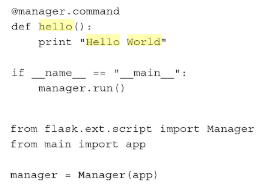
\includegraphics[width=1\textwidth]{figures/3HWFlask.PNG}}
\caption{Contoh Program Flask Hello World}
\label{gambarHWF1}
\end{figure}

Dari gambar \ref{gambarHWF1} kita dapat melihat di sini bahwa Flask-Script mengacu pada dirinya sebagai Manajer, tetapi manajer juga menghubungkan dirinya sendiri dengan aplikasi Flask. Ini berarti kita dapat melakukan apa saja dengan aplikasi Flask hanya dengan menggunakan referensi aplikasi\cite{copperwaite2015learning}.




\section{Error yang Muncul serta Solusinya}
\subsection{Error Flask}
Saat terjadi error muncul di aplikasi Flask? Cara terbaik untuk mengetahuinya ialah dengan mengalaminya secara langsung. Sekarang jalankan aplikasinya, lalu pastikan sudah memiliki dua user yang terdaftar. Kemudian masuk sebagai salah satu user, buka halaman profil dan klik tautan "Edit". Didalam editor untuk profil, coba ubah username dengan username yang sudah dimiliki user lain, dan akan muncul halaman "Internal Server Error"\cite{bae2016efficient}.


\subsection{Halaman Kesalahan Khusus}
Flask memungkinkan aplikasi untuk menentukan halaman kesalahan kustom yang dapat didasarkan pada template, seperti rute reguler. Dua kode kesalahan paling umum adalah 404, yang dipicu ketika klien meminta halaman atau rute yang tidak diketahui, dan 500, dipicu ketika ada pengecualian yang tidak tertangani dalam aplikasi. Cara memberikan penangan khusus untuk dua kesalahan ini menggunakan dekorator app.errorhandler \cite{grinberg2018flask}.

hello.py: halaman kesalahan khusus
\begin{verbatim}
@app.errohandler(404)
def page_not_found(e):
return render_template('404.html'), 404

@app.errohandler(500)
def page_server_error(e):
return render_template('500.html'), 500
\end{verbatim}

Penangan kesalahan mengembalikan respons, seperti fungsi tampilan, tetapi mereka juga perlu mengembalikan kode status numerik yang sesuai dengan kesalahan, yang mudah diterima Flask sebagai nilai pengembalian kedua.
Template yang dirujuk dalam penanganan kesalahan harus ditulis. Template ini harus mengikuti tata letak yang sama dengan halaman biasa, jadi dalam hal ini mereka akan memiliki bilah navigasi dan tajuk halaman yang menunjukkan pesan kesalahan. Cara mudah untuk menulis template ini adalah menyalin templates/user.html ke templates/404.html dan templates/500.html dan kemudian mengubah elemen header halaman dalam dua file baru ini ke pesan kesalahan yang sesuai, tetapi ini akan menghasilkan banyak duplikasi \cite{grinberg2018flask}.




\section{Implementasi dengan menggunakan Flask}
Implementasi web service menggunakan flask web framework, library pandas untuk membaca file csv dan membentuk fitur matrix X dan vektor target y. Penggunan library scikit learn agar dapat menggunakan modul naive bayes, serta untuk melakukan pembagian data training dan testing dengan fungsi train test split. Modul terakhir yang digunakan adalah pickle untuk menyimpan classifier yang telah dibuat ke dalam disk, agar tidak melakukan training berulang-ulang untuk setiap request yang dikirim.

Listing program 1 berfungsi untuk membuat naive bayes classifier, kemudian menyimpannya dengan nama nbp imadiebetspkl agar dapat dipanggil oleh web service. Listing program 2 menampilkan kode pembuatan web service yang diimplementasikan pada fungsi predict, sedangkan Listing program 3 menampilkan contoh kode aplikasi dalam bahasa python yang melakukan request ke web service dengan mengirimkan parameter 'pregn':6,'gluc':148,
'bp':72,'sk':35,'ins':0,
'bmi':33.6,'ped':0.627,'age':50, dimana akan menghasilkan variabel output dengan nilai {'results': [1]} yang berarti positif diabetes \cite{setyawan2017implementasi}.

\begin{verbatim}
Listing program 1. Pembuatan naive bayes classifier
url = 'pima-indians-diabetes.csv'
col_names = ['pregnant', 'glucose', 'bp', 'skin',
'insulin', 'bmi', 'pedigree', 'age', 'label']
pima = pd.read_csv(url, header=None, names=col_names)
feature_cols = ['pregnant', 'glucose', 'bp', 'skin',
'insulin', 'bmi', 'pedigree', 'age']
X = pima[feature_cols]
y = pima.label
X_train, X_test, y_train, y_test =
train_test_split(X, y, stratify=y, test_size=0.25, random_state = 0)
nb = GaussianNB()
nb.fit(X_train, y_train)
pickle.dump(nb, open("nb_pimadiabtes.pkl","wb"))

Listing program 2. Implementasi web service dengan flask
import numpy as np
from flask import Flask, request, abort, jsonify
import pickle
nbclassifier = pickle.load(open("nb_pimadiabtes.pkl","rb"))
app = Flask(__name__)
@app.route('/api', methods=['POST'])
def predict():
data = request.get_json(force = True)
predict_request = [data['pregn'],data['gluc'],data['bp']
data['sk'],data['ins'],data['bmi'],data['ped'],data['age']]
predict_request = np.array(predict_request)
y_result = nbclassifier.predict(predict_request)
output = [int(y_result[0])]
return jsonify(results=output)
if __name__ == '__main__':
app.run(debug = True)

Listing program 3. Contoh kode yang mengakses web service
import json
import requests
url = "http://127.0.0.1:5000/api"

Listing program 3. Lanjutan
data= json.dumps({'pregn':6,'gluc':148,'bp':72,'sk':35,
'ins':0,'bmi':33.6,
'ped':0.627,'age':50})
r = requests.post(url, data)
output = r.json()
\end{verbatim}






\section{Kesimpulan}
Dari berbagai pengertian mengenai bahasa pemograman flask kita dapat simpulkan bahwa bahasa pemograman flask merupakan bahasa pemrograman open source yang banyak digunakan untuk menangani beberapa jenis masalah dalam pemrograman salah satunya membuat suatu framework. flask banyak digunakan untuk meningkatkan kualitas perangkat lunak, produktivitas pengembang, portabilitas program, dan integrasi komponen.

kata lain Flask adalah framework aplikasi web mikro yang ditulis dalam bahasa Python dan berbasiskan toolkit Wekzeug dan template engine Jinja2 dan berlisensi BSD. Pada tahun 2015, versi paling stabil Flask adalah versi 0.10.1. Contoh aplikasi yang menggunakan framework Flask adalah Pinterest, LinkedIn, dan tentu saja halaman web Flask itu sendiri.

Flask dikatakan framework mikro dikarenakan Flask tidak menganggap atau mengharuskan pengembang menggunakan alat atau pustaka tertentu. Flask tidak memiliki lapisan abstrak basis data, validasi form, dan komponen-komponen lainnya yang sudah dimiliki oleh pustaka-pustaka pihak ketiga sebelumnya. Walaupun begitu, Flask mendukung ekstensi yang dapat menambah fitur-fitur seperti layaknya mereka diimplementasikan di dalam Flask itu sendiri. Terdapat ekstensi untuk object-relational mappers, validasi form, upload handlint, dan berbagai teknologi otentikasi terbuka serta peralatan yang berhubungan dengan framework secara umum\cite{solihin2016implementasi}. 

maka dari dibuatnya resume ini kita dapat mengetahui: 
	
\begin{enumerate}
\item mengetahui apa itu flask.
\item wawasan lebih luas tentang flask
\item mengetahui bagaimana cara pembuatan "hello world di flask"
\item mengetahui cara memecahkan masalah pada suatu error code di flask.
\end{enumerate}	


Cukup sekian yang dapat kami sampaikan semoga resume ini dapat bermanfaat bagi pembaca maupun penulis , mohon maaf jika masih banyak kesalahan dalam hal penulisan maupun dalam hal penyampaian materi flask ini, kami harapkan kritik dan saran supaya dapat membuat resume menjadi lebh baik lagi untuk kedepanya kami ucapkan trimakasih banyak  .




